\documentclass[11pt,a4paper]{article}

%Text Color
\usepackage{color}

%Paragraph Spacing
\usepackage{setspace}

%Graphics
\usepackage{graphicx}

%Page Margins
\usepackage{geometry}

%Basic Staff
\usepackage{enumerate}
\usepackage{amsmath}

%Long Table
\usepackage{multicol}
\usepackage{multirow}
\usepackage{longtable}

%URL link
\usepackage{url}

%Appendix
\usepackage[toc,page,title,titletoc,header]{appendix}

%Font sizes
\newcommand{\titlesize}{\fontsize{70pt}{\baselineskip}\selectfont}
\newcommand{\noticesize}{\fontsize{10pt}{\baselineskip}\selectfont}
\newcommand{\intitlesize}{\fontsize{17pt}{\baselineskip}\selectfont}
\newcommand{\licensetitle}{\fontsize{12pt}{\baselineskip}\selectfont}
\begin{document}
    \newcommand{\tabincell}[2]{\begin{tabular}{@{}#1@{}}#2\end{tabular}}
    \begin{titlepage}
        \newgeometry{left=2.7cm,right=2.4cm,top=3.3cm,bottom=2.5cm}
        \begin{figure}[h!]
            \hfill
\includegraphics{Kreogist.png}
        \end{figure}
        \begin{spacing}{2.0}
            \textcolor[rgb]{0.49,0.52,0.55}{\titlesize \\ \textbf{Kreogist Mail\\ Development Documentation\\}}
            \textcolor[rgb]{0.49,0.52,0.55}{\textbf{Software Project Management Plans}\\}
            \textcolor[rgb]{0.49,0.52,0.55}{\textbf{\today}\\}
        \end{spacing}
        \vfill
        \textcolor[rgb]{0.49,0.52,0.55}{
            \begin{flushright}
                Reference Number: KMKOT02.\\
                This document is capable with IEEE Std 1058-1998.
            \end{flushright}
        }
        \restoregeometry
    \end{titlepage}
    \pagenumbering{Roman}
    \thispagestyle{empty}
    \newgeometry{left=2.7cm,right=2.4cm,top=3.3cm,bottom=2.5cm}
    \begin{figure}[h!]
        
\includegraphics[width=2.5cm]{Kreogist.png}
    \end{figure}
    \vspace{4.5cm}
    {
    \noticesize
    \begin{spacing}{0.5}
        \noindent All information provided here is subject to change without notice. Contact Kreogist Dev Team to obtain the latest Kreogist product specifications and roadmaps.\\ \\
        \noindent Kreogist Mail may require enabled hardware, specific software, or services activation. Check with your system manufacturer or retailer.\\ \\
        \noindent No computer system can be absolutely secure. Kreogist does not assume any liability for lost or stolen data or systems or any damages resulting from such losses.\\ \\
        \noindent The products described may contain design defects or errors which may cause the product to deviate from published specifications. Current characterized errata are available on request.\\ \\
        \noindent All the other documents mentioned in this document could be found at the official site of Kreogist Dev Team. Contact Kreogist Dev Team if there's any trouble.\\ \\
        \noindent Intel, Intel Core and the Intel logo are trademarks of Intel Corporation in the U. S. and/or other countries.\\ \\
        \noindent Linux is a trademark of Linus Torvalds in the U. S., other countries, or both.\\ \\
        \noindent Microsoft and Microsoft Windows are trademarks of Microsoft Corporation in the U. S. and/or other countries.\\ \\
        \noindent Macintosh is a trademark of Apple Inc. in the U. S., other countries, or both.\\ \\
        \noindent UNIX is a registered trademark of The Open Group in the U. S. and other countries.\\ \\
        \noindent *Other names and brands may be claimed as the property of others.\\ \\
    \end{spacing}
    \vfill
    \noindent \textbf{First Edition (Jan 2016)}\\ \\
    \noindent This edition applies to Version 0.1 of Kreogist Mail. \\ \\
    \noindent \textbf{Copyright {\copyright} 2016, Kreogist Dev Team. All rights reserved.}\\
    \noindent Permission is granted to copy, distribute and/or modify this document under the terms of the GNU Free Documentation License, Version 1.3 or any later version published by the Free Software Foundation; with no Invariant Sections, no Front-Cover Texts, and no Back-Cover Texts.\\
    \noindent A copy of the license is included in the section entitled "GNU Free Documentation License".
    \noindent Note to government users restricted rights.
    }
    \clearpage
    \thispagestyle{empty}
    {
    \intitlesize
    \noindent Kreogist Dev Team\\ \\ \\
    \noindent \textbf{Kreogist Mail \\
    Development Documentation \\
    Software Project Management Plans}\\ \\ \\
    \today
    }
    \vfill
    \hfill KMKOT02
    \restoregeometry
    \clearpage
    \section*{Signature}
    \addcontentsline{toc}{section}{Signature}
    \noindent The following signature indicates approval of the enclosed Software Project Management Plan.
    \clearpage
    \section*{Revision History}
    \addcontentsline{toc}{section}{Revision History}
    \begin{center}
        \begin{longtable}{|l|l|l|l|}
            \hline
            \multicolumn{1}{|c|}{\textbf{Revision}} & \multicolumn{1}{c|}{\textbf{Version}} & \multicolumn{1}{c|}{\textbf{Description}} & \multicolumn{1}{c|}{\textbf{Date}}\\
            \hline
            \endfirsthead

            \multicolumn{3}{r}%
            \textbf{Continued} \\
            \hline
            \multicolumn{1}{|c|}{\textbf{Revision}} & \multicolumn{1}{c|}{\textbf{Version}} & \multicolumn{1}{c|}{\textbf{Description}} & \multicolumn{1}{c|}{\textbf{Date}}\\
            \hline
            \endhead

            \endfoot

            \hline
            \endlastfoot

            \hline
            KMKOT02 & -001 & Initial commit & Jan. 17th, 2016\\
            \hline
            KMKOT02 & -002 & Internally accepted & Jan. 25th, 2016\\
            \hline
        \end{longtable}
    \end{center}
    \clearpage
    \section*{Preface}
    \addcontentsline{toc}{section}{Preface}
    \paragraph{} This document is an update to the specifications contained in the "Affected Documents" table below. This document is a part of product (project) Kreogist Mail.
    \paragraph{} This document may also contain information that was not previously published.\\
    {
    \noindent \intitlesize \\ Affected Documents \\
    }
    \begin{center}
        \begin{longtable}{|p{10cm}|c|}
            \hline
            \multicolumn{1}{|c|}{\textbf{Document Title}} & \multicolumn{1}{c|}{\textbf{Document Number}} \\
            \hline
            \endfirsthead

            \multicolumn{2}{r}%
            \textbf{Continued} \\
            \hline
            \multicolumn{1}{|c|}{\textbf{Document Title}} & \multicolumn{1}{c|}{\textbf{Document Number}} \\
            \hline
            \endhead

            \endfoot

            \hline
            \endlastfoot

            Kreogist Mail Software Quality Assurance Plan & KMKOT04 \\
            \hline
            Kreogist Mail Software Verification and Validation Plan & KMKOT05 \\
        \end{longtable}
    \end{center}
    {
    \noindent \intitlesize \\ Related Documents\\
    }
    \begin{center}
        \begin{longtable}{|p{10cm}|c|}
            \hline
            \multicolumn{1}{|c|}{\textbf{Document Title}} & \multicolumn{1}{c|}{\textbf{Document Number}} \\
            \hline
            \endfirsthead

            \multicolumn{2}{r}%
            \textbf{Continued} \\
            \hline
            \multicolumn{1}{|c|}{\textbf{Document Title}} & \multicolumn{1}{c|}{\textbf{Document Number}} \\
            \hline
            \endhead

            \endfoot

            \hline
            \endlastfoot

            Kreogist Mail Software Requirement Specification & KMKOT01 \\
            \hline
            Kreogist Mail Software Design Specification & KMKOT03 \\
        \end{longtable}
    \end{center}
    \clearpage
    \addcontentsline{toc}{section}{Table of Contents}
    \tableofcontents
    \clearpage
    \addcontentsline{toc}{section}{List of Figures}
    \listoffigures
    \clearpage
    \addcontentsline{toc}{section}{List of Tables}
    \listoftables
    \clearpage
    \pagenumbering{arabic}
    \setcounter{page}{1}
    \setcounter{table}{0}
    \section{Overview}
        \paragraph{} This section of the document is an introduction to the software development portion of the Kreogist Mail project (��the project��). It will describe the purpose of the project and the objectives that are to be accomplished, the assumptions and constraints that underlie the effort, the deliverables that will be produced by the project, and a summary of the project schedule and budget.
    	\subsection{Project Summary}
			\subsubsection{Purpose, Scope and Objectives}
                \paragraph{} The purpose of the project is to analyze the requirements of, design, implement, and maintain the software for Kreogist Mail (Mail), according to the requirements specified by the client.
                \paragraph{} All activities directly related to the purpose are considered to be in scope. All activities not directly related to the purposes are considered to be out of scope. For example, network availability is not within the scope of this project.
                \paragraph{} The objectives of the project are as follows:
                    \begin{itemize}
                        \item complete the project by the project due date;
                        \item complete the project within budge;
                        \item provide all deliverables identified in section \ref{section:prjdeliver}, i.e.\emph{Project Deliverables} by the project due date;
                        \item fulfill all stated requirements, as in the SRS, of the software product deliverable.
                    \end{itemize}
			\subsubsection{Assumptions and Constraints}
                \paragraph{} The project will be planned with the following assumptions:
                \begin{enumerate}
                    \item this project is a component of a larger project;
                    \item this project will deliver only the Mail components of the larger project;
                    \item initial estimates for the project as provided in this SPMP are +/- 45\%;
                    \item {the software products will be based on the following structures/projects/foundations:
                            \begin{itemize}
                                \item Qt 5.5.1 or later. With its core, gui, widgets and network module installed;
                                \item Kreogist Account system, hosted on bmob.cn;
                                \item Kreogist GUI components from Kreogist Mu.
                            \end{itemize}
                            Mail will be deployed on mainstream desktop Linux release, Mac OS X and Windows.}
                    \item we will be able to acquire the expertise of two outside consultants to assist with the user interface designing.
                    \item this SPMP is submitted as a firm-fixed-price (FFP) bid; the project shall not exceed the
established budget.
                \end{enumerate}
                \paragraph{} Assumptions and constraints of application please check out section \emph{Constraints} and \emph{Assumptions and Dependencies} in \emph{Kreogist Mail Software Requirements Specification}$^{[\ref{ref:srs}]}$.
                \paragraph{} The project will be planned with the following constraints:
                \begin{itemize}
                    \item {budget\\
                            \$0 (software portion only)}
                    \item {time\\
                            1 year}
                    \item {staff
                            \begin{enumerate}
                                \item two outside consultants will be required to assist in the requirements and detail design phases of the project.
                                \item programmers from Github and OSChina open source community to help us improve the quality of the project.
                            \end{enumerate}}
                    \item {maintenance\\
                           The project will receive for a 5-year support. The following version support will be updated in other projects.}
                \end{itemize}
			\subsubsection{Project Deliverables}\label{section:prjdeliver}
                \paragraph{} This project starts at January 4th, 2016. Project should be done before January 31th, 2017. Kreogist Dev Team should delivered the following products:
                    \begin{enumerate}
                        \item Software program and library binaries
                        \item Software source code
                        \item {Software documentation
                                \begin{itemize}
                                    \item Compile documentation
                                    \item Technical Documentation generate with Doxygen
                                \end{itemize}}
                        \item Installation of software program and library binaries on target hardware
                        \item {Project documentation
                                \begin{itemize}
                                    \item Software Requirements Specification (SRS), ID: KMKOT01
                                    \item Software Design Specification (SDS), ID: KMKOT03
                                    \item Software Project Management Plan (SPMP), ID: KMKOT02
                                    \item Software Quality Assurance Plan (SQAP), ID: KMKOT04
                                    \item Software Verification and Validation Plan (SVVP), ID: KMKOT05
                                \end{itemize}}
                    \end{enumerate}
			\subsubsection{Schedule and Budget Summary}\label{section:summary_schedule}
                \paragraph{} The project has the following high-level schedule:
                    \begin{itemize}
                        \item COMP3500 course guide.
                    \end{itemize}
                \paragraph{} The project has a budget of \$0. Once the software product is delivered, annual maintenance costs should be no larger than \$0. Server renting fee is not costed in the budget.
                \paragraph{} The project will be tracked using the Earned Value Management System (EVMS).
		\subsection{Evolution of the Plan}
                \paragraph{} The plan is considered to be a dynamic document and will be updated monthly by default and on an unscheduled basis as necessary. Scheduled updates to the plan will occur once every month, on the last business day of the month.
                \paragraph{} Notification of scheduled and unscheduled updates to the plan will be communicated via e-mail to all project participants according to the section \ref{section:reporting_plan}, i.e.\emph{Reporting Plan}.
                \paragraph{} Once the initial plan is finalized, a baseline of the plan will be created. Changes to the plan will take place against this baseline. The plan will only receive further baselines if significant change in scope occurs.
                \paragraph{} Changes in this information will lead to a new SPMP with a new version number, but with the same status. However, if these changes lead to changes in the milestones planning of the project, described in section \ref{section:schedule}, i.e.\emph{Schedule Allocation}, these changes are discussed with the leader first, before they are incorporated in the document. This will be done during progress meetings. The detailed planning for each phase is described in the appendices of this document. These appendices are updated at different moments in time during the project, but before the start of the phase they refer to.
    \clearpage
    \section{References}\label{section:reference}
        \begin{enumerate}[\texttt{[}1\texttt{]}.]
            \item Kreogist Dev Team. "Kreogist Mail Software Requirements Specification", January, 2016.\label{ref:srs}
            \item Free Software Foundation, "GNU Free Documentation License", See \url{http://www.gnu.org/licenses/fdl.html} (last checked January 13th, 2016), November 3, 2008.\label{ref:fdlv3}
            \item Wikipedia, "Qt (software) - Wikipedia, the free encyclopedia", See \url(https://en.wikipedia.org/wiki/Qt_%28software%29) (last checked January 16th, 2016), January 4, 2016.\label{ref:qt}
            \item Terasoft, Inc.. "Software Project Management Plan (SPMP) for Nirvana National Bank ATM Software Project", May 08, 2004.
            \item IEEE Software Engineering Standards Committee. "IEEE Std 1063-2001, IEEE Standard for Software User Documentation", December 20, 2001.
            \item IEEE Software Engineering Standards Committee. "IEEE Std 830-1998, IEEE Recommended Practice for Software Requirements Specifications", October 20, 1998.
            \item IEEE Software Engineering Standards Committee. "IEEE Std 1016-1998, IEEE Standard for Information Technology--Systems Design--Software Design Descriptions", July 20, 2009.
            \item IEEE Software Engineering Standards Committee. "IEEE Std 1058-1998, IEEE Standard for Software Project Management Plans", December 22, 1998.
            \item IEEE Software Engineering Standards Committee. "IEEE Std 1074-1997, IEEE Standard for Developing Software Life Cycle Processes", 1997.
            \item IEEE Software Engineering Standards Committee. "IEEE Std 1012-1998, IEEE Standard for Software Verification and Validation", 1998.
            \item IEEE Software Engineering Standards Committee. "IEEE Std 828-2005, IEEE Standard for Software Configuration Management Plans", August 12, 2005.
         \end{enumerate}
    \clearpage
    \section{Definitions}
    \paragraph{} This section will define or provide a reference to the definitions of all terms required to properly interpret the Plan. This section shall describe the acronyms and notations used in the Plan.
    \begin{center}
        \begin{longtable}{|p{3cm}|p{9.1cm}|}
            \caption[Definitions]{Definitions, Acronyms \& Abbreviations} \label{grid:abbv} \\
            \hline
            \multicolumn{1}{|c|}{Acronyms} & \multicolumn{1}{c|}{Definition}\\
            \hline
            \endfirsthead

            \multicolumn{2}{r}%
            {\textbf{Continued}} \\
            \hline
            \multicolumn{1}{|c|}{Acronyms} & \multicolumn{1}{c|}{Definition} \\
            \hline
            \endhead

            \endfoot

            \hline
            \endlastfoot
            AD          & Architectural Design  \\
            \hline
            ADD         & Architectural Design Document  \\
            \hline
            ATP         & Acceptance Test Plan  \\
            \hline
            baseline    & a work product that has been formally reviewed and accepted by the involved parties  \\
            \hline
            Client      & Monitor, Agent or Submitter  \\
            \hline
            CM          & Configuration Management  \\
            \hline
            FFP         & Firm-Fixed-Price; a price for fulfilling the contract that will not be under- or over-run \\
            \hline
            IEEE        & Institute of Electrical and Electronics Engineers  \\
            \hline
            milestone   & a scheduled event used to measure progress  \\
            \hline
            MG          & Merge Phase \\
            \hline
            QAM         & Quality Assurance Manager  \\
            \hline
            RA          & Reanalysis Phase \\
            \hline
            SC          & Sprint Check Phase \\
            \hline
            SCMP        & Software Configuration Management Plan  \\
            \hline
            SDS         & Software Design Specification  \\
            \hline
            SM          & Senior Management  \\
            \hline
            SPMP        & Software Project Management Plan (this document)  \\
            \hline
            SQA         & Software Quality Assurance  \\
            \hline
            SQAP        & Software Quality Assurance Plan  \\
            \hline
            SR          & Software Requirements  \\
            \hline
            SRD         & Software Requirements Document  \\
            \hline
            SRS         & Software Requirements Specification  \\
            \hline
            STD         & Software Transfer Document  \\
            \hline
            STP         & Software Testing Plan \\
            \hline
            SUM         & Software User Manual  \\
            \hline
            SVVP        & Software Verification and Validation Plan \\
            \hline
            TR          & Transfer Phase  \\
            \hline
            UTP         & Unit Test Plan  \\
            \hline
            VPM         & Vice Project Manager  \\
            \hline
            VQAM        & Vice Quality Assurance Manager
        \end{longtable}
    \end{center}
    \section{Project Organization}
    	\subsection{External Interfaces}
            \paragraph{} The external structure of the person/companies/organizations having interest in the project is as shown in the following organizational chart. While the
external organization chart suggests "functional" organization, this is for grouping purposes only. The leader of development team is responsible for administration of and dissemination of general organizational information to the team, but does not enjoy a strong reporting relationship with group members.
            \paragraph{} The external organization chart which shows these  relationships is included in Appendix \ref{appendix:org_charts}, i.e.\emph{Organization Charts}.
            \paragraph{} Leader will not incur any direct costs to the project; any administrative costs are integrated into the per-hour cost of the individual resources.
        \subsection{Internal structure, Roles and Responsibilities}\label{section:roles}
            \paragraph{} In the following table, the roles which are distinguished and the person(s) assigned to each role are given. Roles within the group are described in section \ref{section:staff_plan}. i.e.\emph{Staffing plan}.
            \begin{center}
                \begin{longtable}{|p{6.5cm}|p{3cm}|p{4cm}|}
                    \caption[Member Role]{Member Role} \label{grid:staff_roles} \\
                    \hline
                    \multicolumn{1}{|c|}{Role} & \multicolumn{1}{c|}{Name} & \multicolumn{1}{c|}{E-mail}\\
                    \hline
                    \endfirsthead

                    \multicolumn{3}{r}%
                    {\textbf{Continued}} \\
                    \hline
                    \multicolumn{1}{|c|}{Role} & \multicolumn{1}{c|}{Name} & \multicolumn{1}{c|}{E-mail}\\
                    \hline
                    \endhead

                    \endfoot

                    \hline
                    \endlastfoot

                    Team Leader \& Team Member & Haolei Ye & u580415@anu.edu.au\\
                    \hline
                    Project Manager \& Project Manager & Han Wang & u5868791@anu.edu.au \\
                    \hline
                    Quality Assurance Manager \& Team Member & Jinshuai Ma & u5870682@anu.edu.au\\
                    \hline
                    Team Member & & \\
                    \hline
                    Team Member & &
                \end{longtable}
            \end{center}
            \paragraph{} Responsibilities of all the avatar in the project have been listed here:
            \paragraph{Project Manager} Produce and maintain a project management plan and lead the project according to this plan thus ensuring that the product is delivered on time and as specified in the SRS. The PM��s management task includes but is not limited to:
                \begin{itemize}
                    \item Motivating team members;
                    \item Forming teams;
                    \item Checking progress;
                    \item Managing the time budget;
                    \item Gathering all the requirements from outer, manage all the information;
                    \item Providing feedback to the Team Leader through progress reports.
                \end{itemize}
            \paragraph{Quality Assurance Manager} Guarantee that the product will be delivered as agreed and that it is of good quality. This includes but is not limited to:
                \begin{itemize}
                    \item Writing the SQAP and the SVVP;
                    \item Verifying that procedures and standards which are defined in the SQAP and SVVP are adhered to;
                    \item Checking that all project documents are consistent;
                    \item Arranging formal reviews;
                    \item Refactor the unqualified codes and submit to team leader;
                    \item Monitoring and reviewing all testing activities.
                \end{itemize}
            \paragraph{Team Leader} Perform all necessary activities to ensure that a task assigned to a team is performed well and on time. This includes but is not limited to:
                \begin{itemize}
                    \item Planning and coordinating team activities;
                    \item Defining work packages and goals, assigning tasks;
                    \item Motivating team members;
                    \item Check out and sign all the documentation;
                    \item Release the products and give lecture to all end-users.
                \end{itemize}
            \paragraph{Team Member} Perform all necessary activities to ensure that a task assigned to a team is performed well and on time. This includes but is not limited to:
                \begin{itemize}
                    \item Assisting the Team Leader or Project Manager by signaling problems in an early stage;
                    \item Executing plans made by the Team Leader and by the Project Manager;
                    \item Keeping track of time spent on various tasks;
                    \item Following procedures and plans.
                \end{itemize}
    \section{Managerial Process Plans}
    	\subsection{Start-up Plan}
			\subsubsection{Estimation Plan}\label{section:estimation_plan}
                \subsubsection*{Schedule, Cost, and Resource Estimates}
                An estimation chart showing activities, estimated duration, estimated cost, and estimated resource requirements is included in Table \ref{grid:est_chart}.
                \begin{center}
                    \begin{longtable}{|c|p{6cm}|p{2cm}|p{4cm}|}
                        \caption[Estimation Chart]{Estimation Chart} \label{grid:est_chart} \\
                        \hline
                        \multicolumn{1}{|c|}{ID} & \multicolumn{1}{c|}{Task Name} & \multicolumn{1}{c|}{Duration} & \multicolumn{1}{c|}{Resource Names}\\
                        \hline
                        \endfirsthead

                        \multicolumn{4}{r}%
                        {\textbf{Continued}} \\
                        \hline
                        \multicolumn{1}{|c|}{ID} & \multicolumn{1}{c|}{Task Name} & \multicolumn{1}{c|}{Duration} & \multicolumn{1}{c|}{Resource Names}\\
                        \hline
                        \endhead

                        \endfoot

                        \hline
                        \endlastfoot

                        1 & Kreogist Mail project & 1 year & All of the members\\
                        \hline
                        2 & Requirement confirmation & 1 week & Project Manager, Team Leader\\
                        \hline
                        3 & Project Initiation & 1 day & Team Leader, Team Members\\
                        \hline
                        4 & Framework development & 4 weeks & Team Leader, Team Members, Quality Assurance Manager\\
                        \hline
                        5 & Infrastructure development & 4 weeks & Team Leader, Team Members, Quality Assurance Manager\\
                        \hline
                        6 & UI Elements development & 6 months & Team Leader, Team Members, Quality Assurance Manager\\
                        \hline
                        7 & Preference system development & 2 months & Team Leader, Team Members, Quality Assurance Manager\\
                        \hline
                        8 & Plugins development & 2 months & Team Leader, Team Members, Quality Assurance Manager\\
                        \hline
                        9 & Kreogist Account system embedded & 1 months & Team Leader, Team Members, Quality Assurance Manager\\
                        \hline
                        10 & SDK refactor & 2 weeks & Team Leader, Team Members, Quality Assurance Manager\\
                        \hline
                        11 & System test & 1 week & Team Leader, Team Members, Quality Assurance Manager\\
                    \end{longtable}
                \end{center}
                \subsubsection*{Estimation methods}
                \paragraph{} Schedule duration and work estimation for each leaf activity in the Work Breakdown Structure (WBS) will be performed using a combination of the following methods and data sources:
                \begin{enumerate}
                    \item Resource input
                    \item Organizational project history data
                    \item Kreogist project history data
                \end{enumerate}
                \paragraph{} Cost estimation for each activity will be performed by multiplying the amount of work expected by the hourly rate for the resources connected to the activity, multiplied by the percentage of participation that each resource expects to make toward the activity.
                \paragraph{} The resulting estimates for each leaf activity will be rolled-up to produce an estimate for the larger group of activities that the activity is a part of. The highest-level activity in the WBS (after attaching schedule, resource, and cost estimates) will therefore reflect the schedule and cost estimates for the entire project.
                \subsubsection*{Re-stimation methods}
                \paragraph{} When re-estimation is necessary, it will be performed using the following methods and data sources:
                \begin{enumerate}
                    \item Resource input
                    \item Member working input
                \end{enumerate}
                \paragraph{} Once new estimates have been collected, and if schedule is adversely affected (+/- 10\%), organizational project history data will be used to determine whether or not it would be effective
to add additional resources to assist in completing the activity, taking ��roll-on�� time into consideration.
                \subsubsection*{Re-estimation Schedule}
                \paragraph{} Time has been allocated in the schedule for monthly SPMP updates. Necessary updates to the cost, schedule and resource estimates will be included in these SPMP updates. However, such rebaselining will only take place in extreme circumstances, such as when significant scope change has been introduced.
                \paragraph{} The purpose of these monthly updates is to force allocated time toward maintaining the SPMP and to provide a schedule on which stake holders can expect to see updates to the plan. A revised SPMP will be published following each of these update sessions regardless of whether any significant changes have been made so that it is obvious to all involved that the scheduled update has occurred.
                \paragraph{} Impromptu updates to the estimation plan will be made as necessary and communicated to those affected. In particular, detailed explanation is given below to the handling of communication of these update types:
                \begin{itemize}
                    \item Resource
                    \item Cost
                    \item Schedule
                \end{itemize}
                \subsubsection*{Resource}
                \begin{enumerate}
                    \item {If an increase in existing allocation is required
                           \begin{itemize}
                               \item Affected resource
                               \item Project manager
                           \end{itemize}}
                    \item {If addition of internal resources is required
                           \begin{itemize}
                               \item Team Leader
                               \item Project manager
                           \end{itemize}}
                \end{enumerate}
                \subsubsection*{Cost}
                \begin{enumerate}
                    \item {If an increase in costs is required but does not exceed the project budget
                           \begin{itemize}
                               \item Team Leader
                               \item Project Manager
                           \end{itemize}}
                    \item {If an increase in costs is required which exceeds the project budget
                           \begin{itemize}
                               \item Team Leader
                               \item Project Manager
                           \end{itemize}}
                    \item {If a decrease in costs is expected
                           \begin{itemize}
                               \item Project Manager
                           \end{itemize}}
                \end{enumerate}
                \subsubsection*{Schedule}
                \begin{enumerate}
                    \item {If an increase in schedule is required which does not exceed the deadline
                           \begin{itemize}
                               \item Project Manager
                               \item Quality Assurance Manager
                           \end{itemize}}
                    \item {If an increase in schedule is required which exceeds the deadline
                           \begin{itemize}
                               \item Team Leader
                               \item Project Manager
                               \item Quality Assurance Manager
                           \end{itemize}}
                    \item {If a decrease in schedule is expected
                           \begin{itemize}
                               \item Project Manager
                               \item Quality Assurance Manager
                           \end{itemize}}
                \end{enumerate}
			\subsubsection{Staffing plan}\label{section:staff_plan}
                \paragraph{} For role of the member, please check out section \ref{section:roles}, i.e.\emph{Internal structure, Roles and Responsibilities}.
                \subsubsection*{Resource Requirements}
                \paragraph{} Based on initial estimates, the project will require the human resources shown in the table below. Quantity required, estimated work requirement, key work periods and affordable hourly rate ranges are included for each resource type. The key work periods are those periods where the resource will be heavily allocated and should be prepared to have significant (above 20\% working time) availability to the project:
                \begin{center}
                    \begin{longtable}{|p{4.8cm}|p{3.2cm}|p{4cm}|p{0.5cm}|}
                        \caption[Human Resources Requirements]{Human Resources Requirements} \label{grid:human_resource} \\
                        \hline
                        \multicolumn{1}{|c|}{Human Resource Type} & \multicolumn{1}{c|}{Key Periods} & \multicolumn{1}{c|}{Key Project Phase(s)} & \multicolumn{1}{c|}{Qty}\\
                        \hline
                        \endfirsthead

                        \multicolumn{4}{r}%
                        {\textbf{Continued}} \\
                        \hline
                        \multicolumn{1}{|c|}{Human Resource Type} & \multicolumn{1}{c|}{Key Periods} & \multicolumn{1}{c|}{Key Project Phase(s)} & \multicolumn{1}{c|}{Qty}\\
                        \hline
                        \endhead

                        \endfoot

                        \hline
                        \endlastfoot

                        Project Manager & All & All & 1\\
                        \hline
                        Quality Assurance Manager & All & All (but most work up-front during definition) & 1\\
                        \hline
                        Team Leader & All & Requirements, Design, Development & 1\\
                        \hline
                        Team Member & All & Development & 2
                    \end{longtable}
                \end{center}
                \subsubsection*{Attendance at weekly project status meetings}
                \paragraph{} Most staff will be required to attend weekly project status meetings, for which the dates are yet to be determined. All staff identified as "Leads" will be required to attend the meetings. Staff who are in a group underneath a "Lead" will not be required to attend, while staff who have a "Lead" role, or who have no subordinate "Lead" will be required to attend.
                \subsubsection*{Reassignment}
                \paragraph{} All efforts will be made to communicate changes in the key resource requirement dates to leader.
			\subsubsection{Resource Acquisition Plan}
                \paragraph{} All human resources shall be acquired for the purposes of working on the project by the team leader. The team leader must present the resource requirements in detail to project manager and the functional managers of each requested resource; team leader has the ultimate responsibility for approving resources to work on the project.
                \paragraph{} The project manager shall be responsible for acquiring all non-human resources required by the project. The non-human resources identified as being required for the project are:
                \begin{itemize}
                    \item Printing services
                    \item Documentation management
                    \item Software repository
                \end{itemize}
		\subsection{Work Plan}
			\subsubsection{Work activities}\label{section:work_activity}
                \paragraph{} Work activities are illustrated by a work activities table (Table \ref{grid:work_act_chart}).
                \begin{center}
                    \begin{longtable}{|c|p{7cm}|p{2.5cm}|p{2.5cm}|}
                        \caption[Work Activities]{Work Activities} \label{grid:work_act_chart} \\
                        \hline
                        \multicolumn{1}{|c|}{ID} & \multicolumn{1}{c|}{Task Name} & \multicolumn{1}{c|}{Predecessors} & \multicolumn{1}{c|}{Successors}\\
                        \hline
                        \endfirsthead

                        \multicolumn{4}{r}%
                        {\textbf{Continued}} \\
                        \hline
                        \multicolumn{1}{|c|}{ID} & \multicolumn{1}{c|}{Task Name} & \multicolumn{1}{c|}{Predecessors} & \multicolumn{1}{c|}{Successors}\\
                        \hline
                        \endhead

                        \endfoot

                        \hline
                        \endlastfoot

                        1 & Kreogist Mail project & & \\
                        \hline
                        2 & Requirement confirmation & & 3 \\
                        \hline
                        3 & Project Initiation & 2 & 4, 5\\
                        \hline
                        4 & Framework development & 3 & 6\\
                        \hline
                        5 & Infrastructure development & 3 & 6\\
                        \hline
                        6 & UI Elements development & 4, 5 & 7, 8\\
                        \hline
                        7 & Preference system development & 6 & 9 \\
                        \hline
                        8 & Plugins development & 6 & 9 \\
                        \hline
                        9 & Kreogist Account system embedded & 7, 8 & 10\\
                        \hline
                        10 & SDK refactor & 9 & 11 \\
                        \hline
                        11 & System test & 10 & \\
                    \end{longtable}
                \end{center}
			\subsubsection{Schedule Allocation}\label{section:schedule}
                \paragraph{} Schedule allocation is illustrated by a network diagram at figure \ref{figure:net_diagram}.
                \begin{figure}[!h]
                    \centering
                    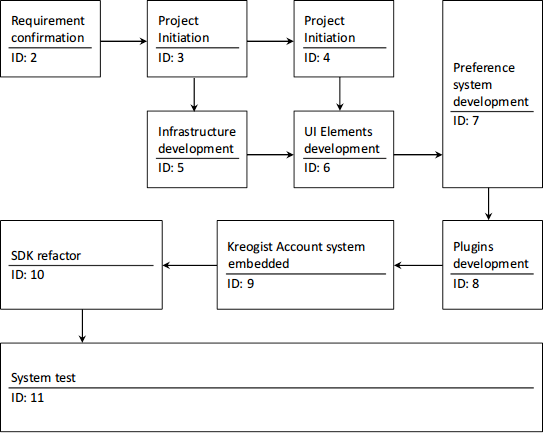
\includegraphics[width=0.618\textwidth]{NetworkDiagram.png}
                    \caption{Network Diagram}\label{figure:net_diagram}
                \end{figure}
		\subsection{Control Plan}
			\subsubsection{Requirements Control Plan}
                \subsubsection*{Requirements tracing}
                \paragraph{} Requirements have all designed in SRS. Before course COMP3500 provides any requirements tracing tools, we will trace the requirements manually. All work effort must be related to a traceable requirement, in order to limit unnecessary work and ensure integrity of the product requirements.
                \subsubsection*{Prioritization}
                When a requirement is entered into the schedule, it is assigned a priority, as follows:
                \begin{itemize}
                    \item 3 = mission critical (product must have)
                    \item 2 = important (should exist, but not absolutely necessary)
                    \item 1 = nice to have (should be present if time permits, but is optional)
                \end{itemize}
                \paragraph{} A requirement��s priority will affect the attention it receives when tradeoffs become necessary, and when changes to requirements are requested. In conjunction with the above, a requirement change priority will also be used to rate the priority of incorporating change to the requirement, as follows:
                \begin{itemize}
                    \item 3 = critical (change must be made to requirement)
                    \item 2 = important (change should be made, but not absolutely necessary)
                    \item 1 = nice to have (change should be made if time permits, but is optional)
                \end{itemize}
                \subsubsection*{Product requirements change control}
                \paragraph{} Changes to product requirements will be considered based on their priority, their point-in-time of introduction within the overall project schedule, the extent of their impact to work products already base-lined as configuration items, and the extent of their impact to in-progress work products.
                \paragraph{} All efforts will be made to incorporate changes to priority 3 requirements. Changes to priority 2 and 1 requirements will be handled only if time permits and/or the customer is willing to negotiate a increase in project budget and schedule.
                \paragraph{} The development model being used for this project is based on up-front solidification of requirements and is appropriate for software products having the profile of the product being developed by this project. Therefore, all requirements change requests should come with the expectation that project schedule and/or budget will be affected if they are introduced after the requirements phase is complete.
                \subsubsection*{Reporting}
                \paragraph{} Assessments produced for each area of assessment listed below above must be communicated to team leader:
                \begin{enumerate}
                    \item product scope
                    \item product quality
                    \item project schedule
                    \item project budget
                    \item project resources
                    \item project risks
                \end{enumerate}
                \paragraph{} Team leader will coordinate necessary resources to approve or reject the requirements change and associated/negotiated increases in budget and schedule. When multiple requirements changes are under consideration at the same time, the requirement-change priority will be used to determine which changes will and will not be implemented, and/or to settle issues of contention.
                \paragraph{} Team leader must be made aware of all requirements changes that are determined to require changes to project schedule, budget or resource requirements occur once the SRS is base-lined. Quantities associated with each of these items must also be reported.
			\subsubsection{Schedule Control Plan}
                \paragraph{} As stated in section \ref{section:summary_schedule}, i.e.\emph{Schedule and Budget Summary}, the project will perform schedule control using the Earned Value Management System (EVMS). In addition, the Critical Path Method (CPM) will be used to control the activities most crucial to completion of the project on-schedule.
                \subsubsection*{Critical Path Method (CPM)}
                \paragraph{} The critical path illustrated by the network diagram (Figure \ref{figure:net_diagram}) shall receive special attention with respect to completion on schedule. Failure to complete these activities within their allotted time will cause slippage of the entire schedule.
                \paragraph{} Bi-weekly examination of the critical path will be undertaken in order to account for activities that enter and leave the critical path as real progress data is entered against the baseline  project schedule.
                \subsubsection*{Activity completion status}
                \paragraph{} In the section \ref{section:estimation_plan}, i.e.\emph{estimation plan}, it is stated that each activity (represented by a work package) estimate shall consist of sub-activity milestones which will be attached to the identification of how complete ("\% complete") a work package is at a given point in time. Activity completion status will be reflected (and only reflected) by the meeting of these sub-activity milestones. Sub-activity milestones will be developed for each activity by the assigned resources as the depth of each activity becomes known. These milestones will be communicated to the project manager, who will work with the resource to attach a "\% complete" value to each milestone so that the progress of each activity may be understood.
                \subsubsection*{Major Milestones}
                \paragraph{} The following major milestones and associated completion identifiers are defined in Table \ref{grid:major_milestone}:
                \begin{center}
                    \begin{longtable}{|c|p{5cm}|p{3cm}|p{4cm}|}
                        \caption[Major Milestone]{Major Milestone} \label{grid:major_milestone} \\
                        \hline
                        \multicolumn{1}{|c|}{ID} & \multicolumn{1}{c|}{Milestone} & \multicolumn{1}{c|}{Date} & \multicolumn{1}{c|}{Complete When...}\\
                        \hline
                        \endfirsthead

                        \multicolumn{4}{r}%
                        {\textbf{Continued}} \\
                        \hline
                        \multicolumn{1}{|c|}{ID} & \multicolumn{1}{c|}{Milestone} & \multicolumn{1}{c|}{Date} & \multicolumn{1}{c|}{Complete When...}\\
                        \hline
                        \endhead

                        \endfoot

                        \hline
                        \endlastfoot

                        1 & Project initiation & & \\
                        \hline
                        2 & Infrastructure complete & & \\
                        \hline
                        3 & Plugins complete & & \\
                        \hline
                        4 & SDK complete & & \\
                        \hline
                        5 & Initial release & & \\
                    \end{longtable}
                \end{center}
                \paragraph{} The arrival of major milestones will be treated specially from an effort data collection perspective. With the completion of each major milestone, all team members will be expected to update their effort data, as per section \ref{section:metrics_collection_plan}, i.e.\emph{Metrics Collection Plan}, so that a milestone performance report may be issued; milestone status and performance data will then be updated on the performance reporting site (see section \ref{section:reporting_plan}, i.e.\emph{Reporting Plan}).
                \subsubsection*{Collection of progress data}
                \paragraph{} At the regular weekly project status meetings, where applicable, the participants will each identify the sub-activity milestones that have been met by the work for which they are responsible for during the period in which the status meeting falls. This information will be correlated with the "\% complete" value attached to the milestone and the latter value will be entered into the project plan.
                \paragraph{} Effort data are collected according to the method outlined in section \ref{section:metrics_collection_plan}, i.e.\emph{Metrics Collection Plan}. These data will be used as inputs into progress measurement analysis.
			\subsubsection{Quality Control Plan}
                \paragraph{} This subsection will describe the mechanisms to be used for measuring and controlling quality of work processes and products. Each of the mechanisms mentioned here are described in more detail in section \ref{section:quality_ensure}, i.e.\emph{Quality Assurance Plan}.
                \subsubsection*{Audits}
                \paragraph{} Audits of work processes will not be conducted on a schedule. However, they will be requested by the team leader and maybe one of the the following:
                \begin{itemize}
                    \item Project Manager
                    \item Quality Assurance Manager
                \end{itemize}
                \paragraph{} When requested, audits will be carried out as specified in section \ref{section:quality_ensure}, i.e.\emph{Quality Assurance Plan}.
                \subsubsection*{Reviews}
                \paragraph{} Regularly scheduled reviews of work products will take place according to the schedule described in section \ref{section:reporting_plan}, i.e.\emph{Reviews and Audits Plan}.
                \subsubsection*{Defect/issue tracking}
                \paragraph{} Defects and other issues will be tracked with Github issue system, providing a central location for defect/issue logging and resolution status.
			\subsubsection{Reporting Plan}\label{section:reporting_plan}
                \paragraph{} This section describes the reporting requirements for the project. Specifically, it identifies the project stakeholders, their generic information requirements, the distribution of items of communication, and the performance reporting data that will be communicated during the project.
                \subsubsection*{Stakeholders}
                \paragraph{} The stakeholders in the project are as follows:
                \begin{itemize}
                    \item Kreogist Dev Team
                    \item Project Manager
                \end{itemize}
                \paragraph{} Ad-hoc communication (communication included in this plan) will take place directly with recipients of the item of communication.Ad-hoc communication with hierarchy levels above the team leader will be made through the team leader. Scheduled communication (communication included in this plan) will take place directly with recipients of the item of communication.
                \subsubsection*{Performance Reporting}
                \paragraph{} The project will report performance to plan with the following metrics:
                \begin{enumerate}
                    \item {Requirements
                        \begin{itemize}
                            \item Requirements change count
                        \end{itemize}}
                    \item {Configuration
                        \begin{itemize}
                            \item Configuration churn
                        \end{itemize}}
                    \item {Quality
                        \begin{itemize}
                            \item Lines of code
                            \item Comment percentage
                            \item Open defects vs. closed defects over time
                        \end{itemize}}
                    \item {Risks
                        \begin{itemize}
                            \item Weekly risk change
                            \item Top 10 risks
                        \end{itemize}}
                \end{enumerate}
                \paragraph{} This information will be available electronically in a format accessible by a web browser supporting the HTTP protocol.
                \subsubsection*{Approvals}
                \paragraph{} The team leader approval signatures are required in order to confirm consent to and validity of this reporting plan.
			\subsubsection{Metrics Collection Plan}\label{section:metrics_collection_plan}
                \paragraph{} This section describes the metrics that will be collected by the project and the methods that will be used to collect them. The metrics collected generally fall into one of the following three categories:
                \begin{itemize}
                    \item Effort
                    \item Reviews
                    \item Change Requests
                \end{itemize}
                \subsubsection*{Effort}
                \paragraph{} Effort metrics will be collected by having project team members write out reports as they work on the project. Each team member will have to write their own report and allocate time to one of the listed categories. Entry should be made at least weekly and preferably more often, especially if the team member is involved in work on more than one category in a week. This will increase the accuracy of data by reducing the impact of time on human memory of effort expended.
                \paragraph{} In order to emphasize the importance of effort metrics collection, a small percentage of every second weekly (i.e. every other week) project status meeting will be dedicated to reviewing effort metrics and those metrics to which effort metrics contribute for each week. Questionable metrics will be clarified at the meetings. The metrics will be summarized during the meeting and the information that is produced from them will be highlighted.
                \subsubsection*{Reviews}
                \paragraph{} Review metrics will be collected from review meeting forms, which will identify each of the reviewed problems as either "errors" or "defects". It will be the responsibility of the review minutes note taker to so identify each reviewed problem on the problem report forms. The note taker will also enter the metrics into the Github issue system.
                \subsubsection*{Change Requests}
                \paragraph{} Change request metrics will be processed by team leader manually.
		\subsection{Risk Management Plan}\label{section:risk_managing_plan}
            \paragraph{} This section mentions a number of possible risks for the project. Also, actions or measures are described to prevent or to reduce the risks.
            \paragraph{} Four categories of risks are identified:
                \begin{itemize}
                    \item Risks with respect to the work to be done;
                    \item Risks with respect to the management;
                    \item Risks with respect to the resources;
                    \item Risks with respect to the customer.
                \end{itemize}
            \paragraph{} The risks for each category are listed below. For each risk, a description, a probability to occur, the action associated and the impact of the risk are given.
            \subsubsection{Risks with respect to the work to be done}
                \paragraph{} We only discuss the most important risks.
                \subsubsection*{Miscommunication}
                \paragraph{Probability} Medium
                \paragraph{Prevention} After a meeting, one group member creates an interview report. Every participant and every person who should have been a participant of the meeting should get a copy of this report. Team members should not hesitate to ask and re-ask questions if things are unclear.
                \paragraph{Correction} When it becomes clear that miscommunication is causing problems, the team members involved and the customer are gathered in a meeting to clear things up.
                \paragraph{Impact} High
                \subsubsection*{Time shortage}
                \paragraph{Probability} High
                \paragraph{Prevention} Care is taken to plan enough spare time.
                \paragraph{Correction} When tasks fail to be finished in time or when they are finished earlier than planned the project planning is adjusted. If time shortage becomes severe, user requirements, which have low priority, are dropped after consultation with the project manager and the customer.
                \paragraph{Impact} High
                \subsubsection*{Design Errors}
                \paragraph{Probability} Medium
                \paragraph{Prevention} The design should be reviewed very critically. The advisor should be consulted frequently on his opinion about the feasibility and the correctness of certain design decisions.
                \paragraph{Correction} When errors in the design are noticed the advisor should be consulted to help correct the design errors as soon as possible. Also all the work, that depends on the faulty design, should be halted until the error is corrected.
                \paragraph{Impact} High
                \subsubsection*{Illness or absence of team members}
                \paragraph{Probability} High
                \paragraph{Prevention} Team members should warn their team leader or the PM timely before a planned period of absence.
                \paragraph{Correction} By ensuring that knowledge is shared between team members, work can be taken over quickly by someone else if a person gets ill. When work needs to be taken over by someone a re- division is made of his other tasks so that the workload does not get too high. Planned absence is dealt with in the planning.
                \paragraph{Impact} Medium
                \subsubsection*{Server crash}
                \paragraph{Probability} Low
                \paragraph{Prevention} All products are stored in the project repository, which is backed up by all members at local.
                \paragraph{Correction} When a product gets lost from its working store it is recovered from the most recent backup.
                \paragraph{Impact} Medium
                \subsubsection{Risks with respect to management}
                \subsubsection*{Illness or sudden absence of the project manager}
                \paragraph{Probability} Low
                \paragraph{Prevention} There are very few things in which the presence of the PM cannot be missed for a short period of time. Nevertheless the project manager will inform the team leader of a planned period of absence in time so that the team leader can prepare to take over.
                \paragraph{Correction} By keeping the team leader up-to-date on the project status he will have enough knowledge to take over in case of illness or absence of the project manager.
                \paragraph{Impact} Low
                \subsubsection{Risks with respect to resources}
                \subsubsection*{Unavailability of the technical advisor when needed}
                \paragraph{Probability} Medium
                \paragraph{Prevention} Meetings with the technical advisor can be planned in advance and time has been reserved in his schedule for counseling the team.
                \paragraph{Correction} A different appointment is made, or another expert is consulted.
                \paragraph{Impact} Medium
                \subsubsection{Risks with respect to the customer}
                \subsubsection*{The customer changes his mind about the requirements}
                \paragraph{Probability} High
                \paragraph{Prevention} It is obviously explained to the customer, that after he has accepted a version of the SRS, the SRS cannot be changed by the customer��s wish only.
                \paragraph{Correction} If the customer changes his mind during the requirement phase his new requirements can be incorporated in the SRS. Procedures described in SQAP detail how the SRS may be changed after approval, and how to implement these changes.
                \paragraph{Impact} High
                \subsubsection*{The customer is not available when needed}
                \paragraph{Probability} Medium
                \paragraph{Prevention} Meetings with the customer can be planned well in advance. The customer has been given room in his schedule for his Software Engineering related work.
                \paragraph{Correction} When the customer is not available, meetings may have to be rescheduled.
                \paragraph{Impact} Medium
                \subsubsection{Summary}
                \paragraph{} It is obvious that problems will occur during the project. To avoid problems the following rules should be followed by all team members:
                \begin{itemize}
                    \item Try to signal problems as early as possible and report them to the PM, so that action can be taken;
                    \item Pay attention to communication and make sure everybody understands the things the same way;
                    \item Focus on the agreed user requirements, which express the wishes of the customer;
                    \item Minimize friction between people by helping and supporting each other;
                    \item Follow guidelines that are posed in SQAP to aid coordination and to ensure product quality.
                \end{itemize}
		\subsection{Project Closeout Plan}
            \paragraph{} This section describes the nature of the activities that will be used to closeout the project when it is completed.
            \paragraph{} As noted in the closure checklist, project participants will be gathered for the purpose of a Post-Performance Analysis (PPA). The PPA allows data to be gathered about their performance and experiences so that project processes may be tuned to improve performance on future projects (see section \ref{section:process_imporve}, i.e.\emph{Process Improvement Plan} for how process improvements will be implemented). The PPA will also be used at the end of project phases (also expanded in section section \ref{section:process_imporve}, i.e.\emph{Process Improvement Plan}).
            \paragraph{} The PPA will be carried out according to the following seven-step process:
            \begin{enumerate}
                \item {PPA meeting invitation will be sent to project participants. The invitation will include an instruction to assemble all available data from the following categories so that it may be collected and archived:
                    \begin{itemize}
                        \item dimensional data for all work products (how many, how big, how often produced, etc.)
                        \item lessons learned (risk logs, correspondence, etc.)
                        \item change requests (requirements, specifications, etc.)
                        \item time and effort data (estimates in hours/dollars for WBS items, networks, schedules, etc.)
                        \item questionnaire responses (based on distributed questionnaire; a different questionnaire for team leaders and team members will be used)
                    \end{itemize}}
                \item Allow sufficient time for the team to assemble their data and formulate responses with a report.
                \item {Assemble the team for a PPA meeting
                    \begin{itemize}
                        \item Before starting, communicate to participants that the meeting is for data collection and not ��finger pointing��
                        \item The meeting will be short and tightly focused on data collection
                    \end{itemize}}
                \item Additional meetings will be held until everyone who has something to contribute (i.e. all sources of information and materials) has made their contribution
                \item {Collected data and material will be categorized into one of the following two categories
                    \begin{itemize}
                        \item Process data
                        \item Product data
                    \end{itemize}}
                \item {Collected material will be categorized into one of the following two categories:
                    \begin{itemize}
                        \item For archive
                        \item For disposal
                    \end{itemize}}
                \item {A concise report of the PPA results will be published to summarize the findings, with the following goals:
                    \begin{itemize}
                        \item The report will link to as many of the archived documents as possible
                        \item The report will be easily accessible to all project managers so that any contained information can be used to augment future projects
                    \end{itemize}}
            \end{enumerate}
    \clearpage
    \section{Technical Process Plans}
        \subsection{Process Model}
            \subsubsection*{List of processes not used}
            \paragraph{} The following IEEE 1074 processes were not used in the Software Life Cycle Process (SLCP) constructed for this project:
            \begin{itemize}
                \item {\textbf{Concept Exploration}\\
                       Since this project is a subproject contracted to Kreogist Dev Team, as part of a larger project initiated by Kreogist Dev Team, we were presented with what was to be delivered. A concept exploration was not necessary because the concept had already been explored by Kreogist Dev Team.}
                \item {\textbf{Retirement}\\
                       Retirement of the software is not within the scope of what Kreogist Dev Team was asked to do. The project only exists for the purpose of delivering Mail application to Kreogist Dev Team.}
            \end{itemize}
            \subsubsection*{List of processes used, but not elaborated}
            \begin{itemize}
                \item {\textbf{Maintenance}\\
                       Requirements for maintenance were provided by Kreogist Dev Team.}
                \item {\textbf{Operation and Support}\\
                       Kreogist Dev Team will operate or support the Mail application.}
            \end{itemize}
            \subsubsection*{Process model diagram}
            \paragraph{} The process model for Mail is our original agile model. It's a kind of Scrum, but we simplified it and focus on product itself. The process model diagram is included as Figure \ref{figure:dev_model}.
            \begin{figure}[h!]
                \centering
                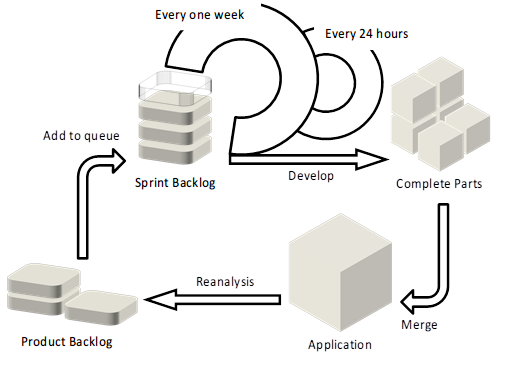
\includegraphics[width=0.618\textwidth]{DevModel.png}
                \caption{Mail Developing Model}\label{figure:dev_model}
            \end{figure}
            \paragraph{} The project is divided into several loop. Each loop will be divided into four phases. These phase are:
            \begin{itemize}
                \item SC (sprint check) phase
                \item TR (transfer) phase
                \item MG (merge) phase
                \item RA (reanalysis) phase
            \end{itemize}
            \paragraph{} In SC, team determine all the backlogs which will be done in this sprint. Once all the backlogs are written on the list, no one could add anything more on the list. In TR, team will ensure that all the parts merge to server should be fully tested and guarantee the quality of the codes. All the modules will be merged to master branch after checking in MG. All of the members should test the product and add new ideas to product backlogs. Documents might be changed at any time of the development.
            \subsubsection*{Individual process diagrams}
            Each of the process boxes on the "Process model diagram" are treated with individual diagrams to overcome the shortcomings of the larger diagram introduced due to layout space. These diagrams are included in Figure \ref{figure:dev_model}.
        \subsection{Methods, Tools, and Techniques}
            \subsubsection*{Development methodology}
            \paragraph{} We will use our own agile development methods, called Agile Incremental Methodology.
            \paragraph{} The decision to use the waterfall methodology is due to the following characteristics of the project:
            \begin{itemize}
                \item The product definition is unstable;
                \item Requirements and implementation of the product are not very clearly understood;
                \item Technical tools and hardware technology are familiar but we don't have any experience or any products could reference;
                \item Agile Incremental Methodology has proven successful for projects of this nature performed by Kreogist Dev Team and the consulting firm we use (Kreogist Mu, Kreogist Cuties) in the past.
            \end{itemize}
            \paragraph{} The Software Project Management Plan (SPMP) shall be based on the IEEE Standard for Software Project Management Plans (IEEE 1058-1998).
            \subsubsection*{Development techniques}
            \paragraph{} The requirement passed down to this project from the larger Kreogist project is that the software be based on an open architecture using a cross-platform platform. This architecture allows us to use object-oriented methods and tools for analysis, design, and implementation. We will use Object Modeling Technique (OMT) for this purpose.
            \subsubsection*{Tools}
            \paragraph{} The following work categories will have their work products satisfied by the identified tools:
            \begin{itemize}
                \item{\textbf{Team member desktop foundation}
                        \begin{enumerate}
                            \item{Microsoft{\textregistered} Windows{\textregistered} platform
                                  \begin{itemize}
                                    \item Microsoft{\textregistered} Windows{\textregistered} 7 Ultimate (64-bit)
                                    \item Oracle{\textregistered} VM VirtualBox [virtual machine support]
                                    \item Microsoft{\textregistered} Office 2010 productivity application suite
                                    \item CTeX suite [LaTeX support]
                                    \item Foxit Reader 3.2 [viewing PDF files]
                                  \end{itemize}}
                            \item{Mac OS X platform
                                  \begin{itemize}
                                    \item Mac OS X 10.9 (Mavericks) / 10.11 (El Capitan)
                                    \item iWork productivity application suite
                                    \item Microsoft{\textregistered} Office for Mac 2016 productivity application suite
                                    \item MacTeX suite [LaTeX support]
                                    \item Adobe Acrobat [creating/viewing PDF files]
                                    \item Preview application [viewing PDF files]
                                  \end{itemize}}
                            \item{Linux platform
                                  \begin{itemize}
                                    \item Ubuntu 14.10
                                    \item LibreOffice 4.4 [Image creating]
                                    \item PDF viewer application [viewing PDF files]
                                  \end{itemize}}
                        \end{enumerate}}
                \item{\textbf{Project management}
                       \begin{enumerate}
                            \item Github repository management
                            \item TechLauncher
                       \end{enumerate}}
                \item{\textbf{Document publishing}
                       \begin{enumerate}
                            \item CTeX suite [document preparation and revision]
                            \item MaxTeX [document preparation and revision]
                       \end{enumerate}}
                \item{\textbf{Quality}
                       \begin{enumerate}
                            \item Sonar@OSC [OSChina provides Sonar Qube quality management platform]
                       \end{enumerate}}
                \item{\textbf{Design}
                       \begin{enumerate}
                            \item Adobe Photoshop CS 6.0 [Image creating]
                            \item Adobe Photoshop CC [Image creating]
                            \item LibreOffice 4.4 [Image creating]
                       \end{enumerate}}
                \item{\textbf{Implementation}
                       \begin{enumerate}
                            \item Qt 5.5 [programming language and object code generation]
                            \item Qt Creator 3.0+ [development tools]
                            \item GNU Debugger [debugging tools]
                            \item Microsoft Visual Studio 2013 [64-bit Windows environment compiler]
                            \item XCode 5/6+ [64-bit Mac OS X environment compiler]
                            \item GNU Compiler Collection [32/64-bit Linux environment compiler, 32-bit Windows environment compiler]
                       \end{enumerate}}
            \end{itemize}
            \subsubsection*{Document distribution}
            \paragraph{} All documents distributed electronically will first be created in the Adobe PDF format using LaTeX PDF compiler.
            \subsubsection*{Change management policy}
            \paragraph{} Once a work product has been finalized and approved, all changes to that work product must be submitted to the project manager via E-mail, where the changes will be reviewed and either approved or denied by the project manager, based on the risk profile and perceived benefit of the change to be made. Changes that are approved may be implemented against the work product, while changes that are denied must not take place against the work product.
            \paragraph{} For internal changes (those changes that originate within the project or within Kreogist Dev Team), the severity and potential impact of the result of not implementing the change will be measured against the disruptiveness of implementing the change. In particular, changes that are 30 working days or less downstream of the approval of the work product that they are changing will be treated more liberally than those that are more than 30 working days downstream.
            \paragraph{} For external changes (those changes that originate outside of the project and outside of Kreogist Dev Team), negotiation will take place with respect to the budget and schedule changes that will be required in order to implement the requested change.
        \subsection{Infrastructure Plan}
            \subsubsection*{Physical server access}
            \paragraph{} All the repository will be hosted on Github. We will make a backup at Git@OSC for emergency backup. All the member will contains a clone for the code repository.
            \subsubsection*{Network configuration}
            \paragraph{} Configuration management will be provided by third party and management by project manager.
            \subsubsection*{Software licensing}
            \paragraph{} Licenses for operating systems and software tools are recycled between projects. We will choose all the open-source license which is capable with GNU General Public License version 2 or later.
        \subsection{Product Acceptance Plan}
            \paragraph{} This section will describe the methods of acceptance for each of the project deliverables identified in section \ref{section:prjdeliver}, i.e.\emph{Project Deliverables}; the headings of this plan relate to the deliverable categories in that section. Acceptance of work products is ultimately achieved when approval is granted by the person with such responsibility, as described in section \ref{section:roles}, i.e.\emph{Internal structure, Roles and Responsibilities}.
            \subsubsection*{Project documentation}
            \paragraph{} All "project documentation" items, with the exception of the SPMP, are approved by the project manager and will be reviewed by both the project manager and the person with lead authority in production of the document to ensure that the document meets all of the requirements of the phase into which it will be fed.
            \paragraph{} The SPMP will be approved by Kreogist Dev Team.
            \subsubsection*{Software program and library binaries}
            \paragraph{} When the software program and library binaries are ready to be installed on the target hardware, the project manager will hold a review session with Kreogist Dev Team steering committee in order to report outstanding known issues with the software, once testing has been completed. The Kreogist Dev Team steering committee will deliver a decision to the project manager on whether or not the list of issues is acceptable for procession with installation. If the list is not acceptable, the Kreogist Dev Team steering committee will work with the project manager to reduce the list of issues to a list that is acceptable to Kreogist Dev Team. Acceptance will occur when this list is satisfactory to the Kreogist Dev Team steering committee.
            \subsubsection*{Installation of software program and library binaries on target hardware}
            \paragraph{} Installation of the software products on the target hardware is the final project deliverable. All the testing will be done with the Kreogist Dev Team members. A review committee will be hold after one platform is fully tested. Acceptance will occur when all the platform is done and there's no known issue during the test.
            \subsubsection*{Software source code}
            \paragraph{} All the source code will be provided by Kreogist Dev Team and released as GNU General Public License version 2 or later on Github even during the development state.
            \subsubsection*{Software documentation}
            \paragraph{} Technical Documentation will be generated with Doxygen from the source code. Kreogist Dev Team should provides a compile documentation for different platforms. Acceptance will occur when the compile documentation could be done without any problems.
            \subsubsection*{Approvals}
            \paragraph{} The team leader approval signatures are required in order to confirm consent to and validity of this reporting plan.
    \clearpage
    \section{Supporting Process Plans}
        \subsection{Verification and Validation Plan}
            \paragraph{} This section briefly describes the Verification and Validation (V\&V) approach for the project. Further detail will be provided by the external Software Verification and Validation Plan (SVVP), when it is developed by Quality Assurance Manager.
            \subsubsection*{Scope}
            \paragraph{} Formal validation and verification will be performed on the following project work products and are listed below in order of occurrence:
                \begin{enumerate}
                    \item Software requirements
                    \item Software architecture
                    \item Software interface design
                    \item Database design
                    \item Implemented software interfaces
                \end{enumerate}
            \paragraph{} The main V\&V activities performed on these work products will be inspections and reviews. Audits may also be performed on request.
            \paragraph{} All other work products will be informally verified and validated to some degree, but they will not receive formal verification and validation from the verification and validation team members.
            \subsubsection*{Responsibilities}
            \paragraph{} The verification and validation team consists of the following resources:
                \begin{itemize}
                    \item Quality Assurance Manager (Lead)
                    \item Team Leader
                    \item All the team members
                \end{itemize}
            \paragraph{} Each of the validation and verification activities are included in the project work activities(see section \ref{section:work_activity}). The specific responsibilities of resources and resource collaborations are identified in section \ref{section:roles}, i.e.\emph{Internal structure, Roles and Responsibilities}.
            \paragraph{} The team "Lead", identified above, has responsibility for focusing and coordinating the V\&V effort of each resource listed in this section and is ultimately responsible for the outcome of the activities of the team.
            \subsubsection*{Tools \& Techniques}
            \paragraph{} Each of the items listed in the "Scope" subsection of this section will be verified and validated to ensure that they account for all items  in the products of the preceding activity. The first item, which has no precedent, will be verified and validated against documented customer meetings to ensure that all requirements are included in the SRS.
            \paragraph{} Tracing will be used to trace the existence of  features between phases back to the original requirements and avoid the introduction of unnecessary work into the products. In particular, the following will be traced:
                \begin{enumerate}
                    \item User requirements to software requirements
                    \item Software requirements to interface requirements
                    \item Architecture requirements to interface requirements
                    \item Interface requirements to database requirements
                    \item Software tests to interface requirements
                    \item Acceptance tests to user requirements
                \end{enumerate}
            \paragraph{} The information produced by tracing will be used during software inspections. Software inspections will ensure that work products are faithfully representing the goals set out for them by the predecessor documents.
            \paragraph{} Black-box and black-white-box-mixing testing will be performed on the implemented software interfaces to ensure that the outputs of each interface are consistent with what is input, based on the interface design.
            \paragraph{} The following tools will be used to assist with V\&V:
                \begin{itemize}
                    \item Valgrind
                    \item Github issue repository tracing system.
                \end{itemize}
            \subsubsection*{Reviews}
            \paragraph{} Regular peer reviews will be held to review in-progress work products. The procedure for scheduling these reviews is included in section \ref{section:review}, i.e.\emph{Reviews and Audits Plan}.
            \subsubsection*{Reporting}
            \paragraph{} For each verification and validation of a configuration item, a corresponding report will be issued by the team. The report will consist of:
                \begin{itemize}
                    \item unique report ID
                    \item problems discovered, and, if known, corresponding solutions
                    \item acceptance or rejection of the item (rejections should be explained)
                \end{itemize}
        \subsection{Documentation Plan}\label{section:documentation_plan}
            \paragraph{} This section describes the documentation plan for the project��s deliverable and non -deliverable documentation work products. All deliverable work products appear in section \ref{section:prjdeliver}, i.e.\emph{Project Deliverables}.
            \paragraph{}The table headings are defined as follows:
                \begin{itemize}
                    \item \textbf{Document}: the documentation work product described by the remaining columns in the row
                    \item \textbf{ID}: the documentation work product identified number
                    \item \textbf{Template/Standard (T/S)}: the template or standard on which the document is based (may be organizational or external). See section \ref{section:reference}, i.e.\emph{References} for template/standard details.
                    \item \textbf{Reviewer}: the person responsible for reviewing the document.
                    \item \textbf{Distribution list}: expected recipients of the review copies and baseline versions of the document
                \end{itemize}
            \subsubsection*{Deliverable documentation work products}
                \begin{center}
                    \begin{longtable}{|p{4cm}|c|p{1.6cm}|p{1.6cm}|p{2.8cm}|}
                        \caption[Documentation Delivered List]{Documentation Delivered List} \label{grid:document_delivered} \\
                        \hline
                        \multicolumn{1}{|c|}{Document} & \multicolumn{1}{|c|}{ID}& \multicolumn{1}{c|}{T/S} & \multicolumn{1}{c|}{Reviewer} & \multicolumn{1}{c|}{Distribution list}\\
                        \hline
                        \endfirsthead

                        \multicolumn{5}{r}%
                        {\textbf{Continued}} \\
                        \hline
                        \multicolumn{1}{|c|}{Document} & \multicolumn{1}{|c|}{ID}& \multicolumn{1}{c|}{T/S} & \multicolumn{1}{c|}{Reviewer} & \multicolumn{1}{c|}{Distribution list}\\
                        \hline
                        \endhead

                        \endfoot

                        \hline
                        \endlastfoot

                        Software Requirements Specification (SRS)           & KMKOT01 & IEEE Std 830-1998  & Team Leader & Preparer, Reviewer, Project Manager, Team member \\
                        \hline
                        Software Design Specification (SDS)                 & KMKOT02 & IEEE Std 1016-1998 & Team Leader & Preparer, Reviewer, Project Manager, Team member \\
                        \hline
                        Software Project Management Plan (SPMP)             & KMKOT03 & IEEE Std 1058-1998 & Team Leader & Preparer, Reviewer, Project Manager \\
                        \hline
                        Software Quality Assurance Plan (SQAP)              & KMKOT04 & IEEE Std 730-2002  & Team Leader & Preparer, Reviewer, Project Manager \\
                        \hline
                        Software Verification and Validation Plan (SVVP)    & KMKOT05 & IEEE Std 1012-1998 & Team Leader & Preparer, Reviewer, Project Manager, Team member \\
                    \end{longtable}
                \end{center}
        \subsection{Quality Assurance Plan}\label{section:quality_ensure}
            \paragraph{} This section will describe the plans for assuring that the quality of delivered work products is consistent with what is expected for the project. Further detail will be provided by the external Software Quality Assurance Plan (SQAP), when it is developed by Quality Assurance Manager.
            \subsubsection*{Scope}
            \paragraph{} The processes used to create the following products will be tracked:
            \begin{enumerate}
                \item Software Requirements Specification (SRS), ID: KMKOT01
                \item Software Design Specification (SDS), ID: KMKOT02
                \item Software Project Management Plan (SPMP), ID: KMKOT03
                \item Software Quality Assurance Plan (SQAP), ID: KMKOT04
                \item Software Verification and Validation Plan (SVVP), ID: KMKOT05
                \item Software product object code
                \item Software product binaries
                \item End-user documentation
            \end{enumerate}
            \subsubsection*{Reviews}
            \paragraph{} Quality reviews will ensure that documentation products adhere to the standards on which they are based (as per section \ref{section:documentation_plan}), and that non-documentation work products adhere to the plans/designs laid out by their input prerequisites.
            \paragraph{} Quality reviews of in-scope documentation work products will be conducted once the products are complete. Reviews of in-scope non-documentation work products will take place weekly during the periods that their production is active.
            \paragraph{} Each quality review will be in a meeting format and will require the attendance of the following participants:
            \begin{itemize}
                \item Team Leader
                \item Project Manager
                \item Quality Assurance Manager
            \end{itemize}
            \paragraph{} In addition, the Lead team members of teams having involvement in the production of work products must attend.
            \paragraph{} A closure review will be held after all work products have been delivered. This review will be in a meeting format and will be for the purpose of gathering "lessons learned", and identifying process improvement opportunities.
            \subsubsection*{Risk Management}
            \paragraph{} SQA will assist in the following risk factors:
            \begin{itemize}
                \item \textbf{Project processes}: by ensuring process adherence, SQA will help prevent this risk factor from materializing
                \item \textbf{Requirements complete and clear}: by reviewing the SRS for adherence to the standard, SQA will assist in preventing this risk factor from materializing
                \item \textbf{Quality assurance approach}: although this risk item will depend on the quality of SQA itself, the fact that a documented approach exists should limit this risk factor to a Medium rating
            \end{itemize}
            \subsubsection*{Record storage}
            \paragraph{} All SQA records will be stored in the project repository by Quality Assurance Manager.
        \subsection{Reviews and Audits Plan}\label{section:review}
            \paragraph{} This section will describe the schedule, resources, methods and procedures used to conduct project reviews and audits.
            \paragraph{} Since multiple project managers are referred to in the following tables, Manager will be used to refer to the project manager on the project described by this SPMP.
            \paragraph{} All review agendas and minutes are subject to handling as described in the documentation plan in section \ref{section:documentation_plan}, i.e.\emph{Documentation Plan}.
            \paragraph{} The table headings are defined as follows:
            \begin{itemize}
                \item \textbf{Review/Audit}: the review/audit type described by the remaining columns in the row
                \item \textbf{Schedule}: the schedule basis for the review meetings
                \item \textbf{Resources}: the resources required to participate in the review
            \end{itemize}
            \subsubsection*{Review and Audits List}
                \begin{center}
                    \begin{longtable}{|p{5cm}|p{3.2cm}|p{5cm}|}
                        \caption[Review and Audits List]{Review and Audits List} \label{grid:review_audits_list} \\
                        \hline
                        \multicolumn{1}{|c|}{Review/Audit} & \multicolumn{1}{|c|}{Schedule}& \multicolumn{1}{c|}{Resources} \\
                        \hline
                        \endfirsthead

                        \multicolumn{3}{r}%
                        {\textbf{Continued}} \\
                        \hline
                        \multicolumn{1}{|c|}{Review/Audit} & \multicolumn{1}{|c|}{Schedule}& \multicolumn{1}{c|}{Resources} \\
                        \hline
                        \endhead

                        \endfoot

                        \hline
                        \endlastfoot

                        \multicolumn{3}{|c|}{\textbf{Joint acquirer/supplier reviews}}\\
                        \hline
                        Software project review & 6th month, 12th month & Kreogist Dev Team\\
                        \hline
                        Steering committee progress review & Weekly & Team Leader, Quality Assurance Manager and Team Members\\
                        \hline
                        \multicolumn{3}{|c|}{\textbf{Management progress reviews}}\\
                        \hline
                        Tutor Meeting & Twice a month & Kreogist Dev Team \\
                        \hline
                        \multicolumn{3}{|c|}{\textbf{Developer peer reviews}}\\
                        \hline
                        Requirements peer reviews & Weekly & Team Leader, Team members\\
                        \hline
                        Design peer reviews & Weekly & Team Leader, Team members\\
                        \hline
                        Implementation peer reviews & Daily & Team Leader, Team members\\
                        \hline
                        \multicolumn{3}{|c|}{\textbf{Quality assurance audits}}\\
                        \hline
                        Project documentation reviews & Weekly, during periods when project documentation is being created & Team Leader, Team Members and Project Manager\\
                        \hline
                        \multicolumn{3}{|c|}{\textbf{Acquirer-conducted reviews}}\\
                        \hline
                        Software acceptance review & Once & Kreogist Dev Team\\
                    \end{longtable}
                \end{center}
        \subsection{Problem Resolution Plan}\label{section:problem_resolution_plan}
            \subsubsection*{Problem reporting}
            \paragraph{} All problems must be reported to the project manager using the problem reporting form designated for use on the project. When complete, the form should be submitted electronically, via e-mail.
            \subsubsection*{Problem analysis}
            \paragraph{} Reported problems will be analyzed to determine the risk they pose to the project, and the short- and long-term impact they will have on project resources, schedule, and budget.
            \paragraph{} Problem reports will be analyzed against the Risk Categorization Table (see section \ref{section:risk_managing_plan}, i.e.\emph{Risk Management Plan}). If an existing risk��s status is determined to require elevation due to the problem report, this will be done. If the problem poses a new risk to the project, a new risk entry will be made to the Risk Categorization Table.
            \paragraph{} Depending on the nature and reach of the problem, the appropriate team members will be engaged to properly analyze the problem, determine resolution steps, and estimate time required to resolve the problem. Mandatory participants are:
            \begin{itemize}
                \item Team Leader
                \item One of the Team Member
            \end{itemize}
            \paragraph{} As time is more important than budget or resources on this project, emphasis will be on determining the problem's impact on project schedule. This must include an analysis of the impact of diverting resource attention away from planned project activities toward resolving problems.
            \paragraph{} Root cause analysis will be performed on the problem if time permits and/or a serious process flaw is suspected to be the cause or to have contributed to the cause. Associated possible process improvements will be documented by Quality Assurance Manager. See section \ref{section:process_imporve}, i.e.\emph{Process Improvement Plan} for process improvement plans.
            \subsubsection*{Problem prioritizing}
            \paragraph{} Based on analysis of the problems, and given that time is the most important factor on this project, the problems will be prioritized based on the extent of their impact to schedule if they are allowed to persist. The problems will be classified as follows:
            \begin{itemize}
                \item Critical (highest priority): problem will impact and/or has impacted delivery time of activities on the critical path
                \item High: problem has impacted and continues to impact delivery time of activities not on the critical path; will affect critical path if not resolved
                \item Medium: problem has an ongoing impact to schedule but is not expected to affect critical path
                \item Low (lowest priority): problem has/had a one-time impact, and/or is so minor that critical path will never be affected
            \end{itemize}
            \subsubsection*{Problem processing}
            \paragraph{} All the problems will be state on the issue list on Github issue tracking system. Once a issue is submitted, we will give it some labels, highlight it as bug, problem, etc. Quality Assurance Manager will record it. One of the team member will be allocate as assignee. The assignee will be responsible for the issue.
            \subsubsection*{Roles}
            \paragraph{} The following table illustrates the roles of project team members in the problem resolution process:
                \begin{center}
                    \begin{longtable}{|p{5cm}|p{8.2cm}|}
                        \caption[Roles of Members in Problem Processing]{Roles of Members in Problem Processing} \label{grid:issue_role} \\
                        \hline
                        \multicolumn{1}{|c|}{Team Function} & \multicolumn{1}{|c|}{Role(s)}\\
                        \hline
                        \endfirsthead

                        \multicolumn{2}{r}%
                        {\textbf{Continued}} \\
                        \hline
                        \multicolumn{1}{|c|}{Team Function} & \multicolumn{1}{|c|}{Role(s)}\\
                        \hline
                        \endhead

                        \endfoot

                        \hline
                        \endlastfoot

                        \vfill Team Leader & {\begin{itemize}
                                            \item Allocate issue to team member.
                                            \item Authors problem summary.
                                            \item Check the bug and modified the code.
                                       \end{itemize}}\\
                        \hline
                        \vfill Team Member & {\begin{itemize}
                                            \item Check the bug and modified the code.
                                            \item Give the report to team leader.
                                       \end{itemize}}\\
                        \hline
                        \vfill Quality Assurance Manager & {\begin{itemize}
                                            \item Must participate in problem resolution meetings.
                                            \item Record all the solving process.
                                       \end{itemize}}\\
                        \hline
                        \vfill Project Manager & {\begin{itemize}
                                            \item Manage/modify the documentation when necessary.
                                       \end{itemize}}\\
                    \end{longtable}
                \end{center}
        \subsection{Process Improvement Plan}\label{section:process_imporve}
            \paragraph{} This section describes plans for process improvements obtained during problem resolution and through periodic assessment of the project through PPAs.
            \subsubsection*{Post-performance analysis}
            \paragraph{} Post-Performance Analysis (PPA) allows data to be gathered about their performance and experiences so that project processes may be tuned to improve performance on future projects. The PPA will be carried out according to the following seven-step process:
            \begin{enumerate}
                \item {PPA meeting invitation will be sent to project participants. The invitation will include an instruction to assemble all available data from the following categories so that it may be collected and archived:
                    \begin{itemize}
                        \item dimensional data for all work products (how many, how big, how often produced, etc.)
                        \item lessons learned (risk logs, correspondence, etc.)
                        \item change requests (requirements, specifications, etc.)
                        \item time and effort data
                    \end{itemize}}
                \item Allow sufficient time for the team to assemble their data and formulate responses to the questions on the questionnaire.
                \item {Assemble the team for a PPA meeting
                    \begin{itemize}
                        \item Before starting, communicate to participants that the meeting is for data collection and not "finger pointing".
                        \item The meeting will be short and tightly focused on data collection
                    \end{itemize}}
                \item Additional meetings will be held until everyone who has something to contribute (i.e. all sources of information and materials) has made their contribution.
                \item Collected data and material will be categorized into one of the following two categories: Process data and Product data.
                \item Collected material will be categorized into one of the following two categories: For archive and For disposal.
                \item {A concise report of the PPA results will be published to summarize the findings, with the following goals:
                    \begin{itemize}
                        \item The report will link to as many of the archived documents as possible
                        \item The report will be easily accessible to all project managers so that any contained information can be used to augment future projects
                    \end{itemize}}
            \end{enumerate}
            \paragraph{} The PPA procedure will be used to produce process improvements based on input from participants of project phases the have closed. Any project process improvements that may benefit the ongoing performance of this project will be considered for implementation so that they may benefit the remaining project phases. Potential changes to organizational processes that may produce benefit from PPA input will be documented and deferred for analysis independently of this project.
            \subsubsection*{Problem resolution input}
            \paragraph{} Project process improvements are those that result from the problem resolution efforts described in section \ref{section:problem_resolution_plan}, i.e.\emph{Problem Resolution Plan}. If a root cause analysis is performed and justified process improvements are identified, Quality Assurance Manager will work with the project manager and other key resources directly involved with the process in question to develop changes to the problematic process. If an organizational process is at fault, a temporary workaround will be devised by the same participants which will last for the duration of the project. The problems and temporary workarounds will be documented so that the organizational process that caused the problem can be inspected to determine whether the changes used in this project may be of benefit to the organizational process. If the workaround was only of particular application to the current project, the documentation will be stored in the project repository so that future project managers will be aware of changes required in the process for projects of a similar nature in future.
            \subsubsection*{Other process improvements}
            \paragraph{} Process improvements, while the project is in progress, will not  normally result from anything other than PPAs and problem resolution input for this project in order to keep the project focused. However, any suggestions for process improvements may be forwarded to the project manager at any time. Suggestions that are well-substantiated and supported by metrics may be considered for implementation in mid-project.
    \section{Additional Plans}
        \paragraph{} There are no additional plans.
    \clearpage
    \appendix
    \addcontentsline{toc}{section}{Appendices}\markboth{APPENDICES}{}
    \begin{subappendices}
        \section{Organization Charts}\label{appendix:org_charts}
    \end{subappendices}
\end{document}
